% !TeX document-id = {20b2fa36-dff4-44d5-9bdf-bd32e1c0a57a}
% !TeX TXS-program:compile = txs:///pythontex
\documentclass{mwart}
\usepackage[utf8]{inputenc}
\usepackage{polski}
\usepackage{lmodern,microtype}
\usepackage{tikz}
\usepackage{pythontex}
\usetikzlibrary{trees}
\usetikzlibrary{shadows}
\usepackage[hidelinks, breaklinks, pdfusetitle, pdfdisplaydoctitle]{hyperref}
\usepackage{float}
% Autorzy i metadane
\author{Michał Anczykowski\and Daria Grzelak\and Jan Ratajczyk}
\title{Projekt zespołowy --- opracowanie zadania z prawdopodobieństwa}
\date{\today}
% Początek dokumentu
\begin{document}
\begin{pycode}
import sympy as sp
\end{pycode}
\maketitle
Celem niniejszego projektu jest opracowanie jednego ze starych zadań z matury rozszerzonej z~matematyki. Jest to zadanie 11 z~matury z~2~czerwca~2023~roku w~formule 2015, a~jego treść jest następująca:

\begin{quote}
W pudełku umieszczono $n$~kul ($n \geq 3$), wśród których dokładnie 2~kule są czarne, a~pozostałe kule są białe. Z~tego~pudełka losujemy jedną kulę i~odkładamy ją na bok. Jeżeli wylosowana kula jest biała, to do~pudełka wrzucamy kulę czarną, a~gdy wylosowana kula jest czarna, to do~pudełka wrzucamy kulę białą. Po przeprowadzonej w~ten~sposób zmianie zawartości prawdopodobieństwo wylosowania kuli białej z~tego~pudełka jest równe $\frac{37}{50}$. Oblicz $n$\footnote{Pełen arkusz można znaleźć na stronie \href{https://arkusze.pl/maturalne/matematyka-2023-czerwiec-matura-stara-rozszerzona.pdf}{Arkusze.pl}.}.
\end{quote}

\section{Rozwiązanie dla ścisłej treści zadania}
Ze względu na trudności związane z parametryzacją zadania, które opiszemy poniżej, najpierw przedstawimy rozwiązanie konkretnie dla treści tego zadania.

Na początek należy rozrysować drzewko przedstawiające wszystkie możliwości wylosowania kul.

\begin{figure}[h]
	\centering
	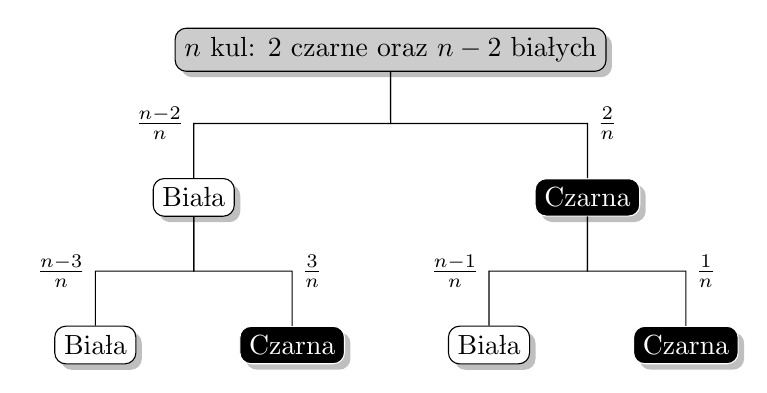
\begin{tikzpicture}[scale=1.25, edge from parent fork down]
		\node [rounded corners, drop shadow, fill=gray!40, draw]{$n$ kul: 2 czarne oraz $n - 2$ białych} [sibling distance=4cm]
			child {node [rounded corners, drop shadow, draw, fill=white] {Biała} [sibling distance = 2cm]
			child {node [rounded corners, drop shadow, draw, fill=white] {Biała}
			edge from parent node [left] {$\frac{n-3}{n}$}
			}
			child {node [rounded corners, drop shadow, draw=white, fill=black] {\textcolor{white}{Czarna}}
			edge from parent node [right] {$\frac{3}{n}$}
			}
			edge from parent node [left] {$\frac{n-2}{n}$}
			}
			child {node [rounded corners, drop shadow, draw=white, fill=black] {\textcolor{white}{Czarna}} [sibling distance = 2cm]
			child {node [rounded corners, drop shadow, draw, fill=white] {Biała}
			edge from parent node [left] {$\frac{n-1}{n}$}
			}
			child {node [rounded corners, drop shadow, draw=white, fill=black] {\textcolor{white}{Czarna}}
			edge from parent node [right] {$\frac{1}{n}$}
			}
			edge from parent node [right] {$\frac{2}{n}$}
			};
	\end{tikzpicture}
\end{figure}

Następnie należy sprawdzić, jakie jest prawdopodobieństwo wylosowania w ostatecznym rozrachunku kuli białej. Aby to zrobić, należy pomnożyć prawdopodobieństwa na jednej gałęzi, a następnie dodać wszystkie z gałęzi.

\begin{equation}
\frac{n-2}{n}\cdot\frac{n-3}{n}+\frac{2}{n}\cdot\frac{n-1}{n} = \frac{n^2-3n+4}{n^2}
\end{equation}

Następnie należy rozwiązać równanie:

\begin{equation}
\frac{n^2-3n+4}{n^2} = \frac{37}{50}
\end{equation}

Możemy je rozwiązać przy pomocy biblioteki Pythona Sympy.
\begin{pycode}
n=sp.Symbol('n', real=True)
równanie = sp.Eq((n**2-3*n+4)/(n**2), (37/50))
rozwiązanie=sp.solveset(równanie, n)
print('Zwrócone rozwiązania to: ' + str(rozwiązanie))
\end{pycode}

Następnie należy sprawdzić, które z rozwiązań są liczbami naturalnymi.

\begin{pycode}
naturalne=[]
for x in rozwiązanie:
	if(x>0 and x//1==x):
		naturalne.append(int(x))
string='Po sprawdzeniu przez Pythona wiadomo, że liczby naturalne stanowiące rozwiązanie równania to: '

for y in naturalne:
	string+=str(y)
string+='.'
print(string)
\end{pycode}

Dla tego przykładu $10$ to jedyna liczba naturalna stanowiąca rozwiązanie zadania, zatem $n = 10$.

\section{Parametryzacja zadania – wariant 1}
W pierwszym wariancie parametryzacji, bardziej zgodnym z treścią zadania, umożliwimy użytkownikowi dodanie wybranej ilości kul czarnych oraz wybranego prawdopodobieństwa wylosowania kuli białej. Liczba kul czarnych musi być liczbą naturalną równą minimum 1 (inaczej program automatycznie ustawi tę liczbę jako 2), a prawdopodobieństwo wylosowania kuli białej musi być liczbą wymierną pomiędzy 0 i 1 (inaczej program automatycznie ustawi tę liczbę jako $\frac{37}{50}$).

\begin{pycode}
czarnekule=input('Podaj ilość czarnych kul: )
licznik=1
mianownik=2


if not (czarnekule>=1 and czarnekule//1==czarnekule):
	czarnekule=2
if not(licznik/mianownik>=0 and licznik/mianownik<=1):
	licznik=37
	mianownik=50

\end{pycode}

Ustawione zmienne prezentują się następująco:

\begin{itemize}
\item liczba kul czarnych: \py{czarnekule},
\item prawdopodobieństwo wylosowania kuli białej: $\frac{\py{licznik}}{\py{mianownik}}$
\end{itemize}

Następnie, tak jak wcześniej, rysujemy drzewko, tylko że z odpowiednią parametryzacją związaną z ilością czarnych kul:

\begin{figure}[h]
	\centering
	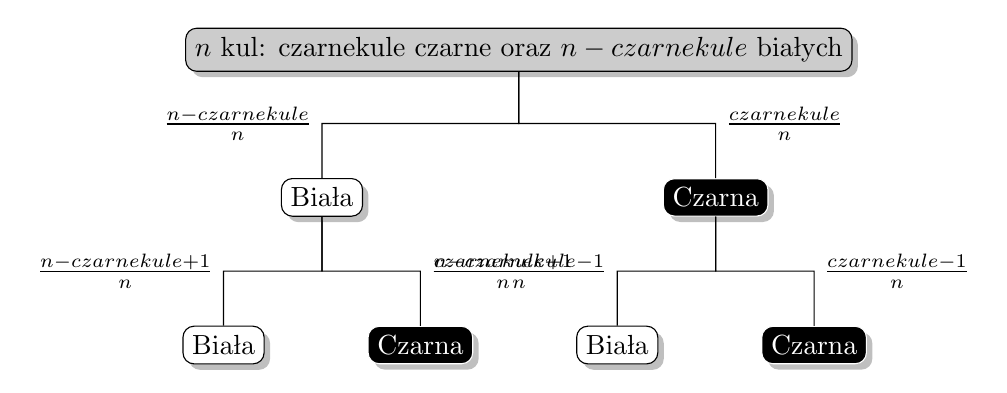
\begin{tikzpicture}[scale=1.25, edge from parent fork down]
		\node [rounded corners, drop shadow, fill=gray!40, draw]{$n$ kul: \py{czarnekule} czarne oraz $n - \py{czarnekule}$ białych} [sibling distance=4cm]
			child {node [rounded corners, drop shadow, draw, fill=white] {Biała} [sibling distance = 2cm]
			child {node [rounded corners, drop shadow, draw, fill=white] {Biała}
			edge from parent node [left] {$\frac{n-\py{czarnekule+1}}{n}$}
			}
			child {node [rounded corners, drop shadow, draw=white, fill=black] {\textcolor{white}{Czarna}}
			edge from parent node [right] {$\frac{\py{czarnekule+1}}{n}$}
			}
			edge from parent node [left] {$\frac{n-\py{czarnekule}}{n}$}
			}
			child {node [rounded corners, drop shadow, draw=white, fill=black] {\textcolor{white}{Czarna}} [sibling distance = 2cm]
			child {node [rounded corners, drop shadow, draw, fill=white] {Biała}
			edge from parent node [left] {$\frac{n-\py{czarnekule-1}}{n}$}
			}
			child {node [rounded corners, drop shadow, draw=white, fill=black] {\textcolor{white}{Czarna}}
			edge from parent node [right] {$\frac{\py{czarnekule-1}}{n}$}
			}
			edge from parent node [right] {$\frac{\py{czarnekule}}{n}$}
			};
	\end{tikzpicture}
\end{figure}

Następnie należy ułożyć równanie, tak jak wcześniej:

\begin{equation}
\frac{n-\py{czarnekule}}{n}\cdot\frac{n-\py{czarnekule+1}}{n}+\frac{\py{czarnekule}}{n}\cdot\frac{n-\py{czarnekule-1}}{n} = \frac{\py{licznik}}{\py{mianownik}}
\end{equation}

Ponownie skorzystamy z biblioteki Sympy do rozwiązania równania.

\begin{pycode}
n=sp.Symbol('n', real=True)

równanie2=sp.Eq(((n-czarnekule)*(n-czarnekule-1))/(n**2)+((czarnekule)*(n-czarnekule+1))/(n**2), (licznik/mianownik))

rozwiązanie2=sp.solveset(równanie2, n)

if not type(rozwiązanie)==sp.sets.sets.EmptySet:
	print('Istnieją rzeczywiste rozwiązania równania i są to: ' + str(rozwiązanie2) +'. Sprawdźmy, które z nich są liczbami naturalnymi nie mniejszymi od liczby kul czarnych.')

	naturalne2=[]
	for x in rozwiązanie2:
		if(x//1==x and x>=czarnekule):
			naturalne2.append(int(x))
	if len(naturalne2)==1:
		print('Jest jedno rozwiązanie spełniające warunki: ' + str(naturalne2[0]) + '. Tyle jest kul w pudełku.')
	elif len(naturalne2)>1:
		print('Jest więcej rozwiązań spełniających warunki. Są to: ')
		for y in naturalne2:
			print(str(y)+', ')
		print(' więc liczbą kul w pudełku jest któraś z tych liczb.')
	else:
		print('Żadne z rozwiązań nie jest liczbą naturalną nie mniejszą niż ilość czarnych kul. Oznacza to, że z podanymi danymi zadanie nie ma rozwiązań.')
else:
	print('Nie ma rzeczywistych rozwiązań równania – zmień dane!')
\end{pycode}

\end{document}